% !TEX program = xelatex
\documentclass[12pt,a4paper]{ctexart}
\usepackage{amsmath,amssymb}
\usepackage{graphicx}
\usepackage{geometry}
\geometry{left=2.5cm,right=2.5cm,top=2.5cm,bottom=2.5cm}
\usepackage{listings}
\usepackage{xcolor}
\usepackage{unicode-math}
\setmainfont{Times New Roman}
\setmathfont{XITS Math}
\usepackage{fontspec}
\setmonofont{Consolas}   % 设置等宽字体为 Consolas
\usepackage{float}
\usepackage{caption}
\usepackage{booktabs}
\usepackage{array}
\usepackage{hyperref}
% MATLAB 代码风格
\definecolor{matlabgreen}{rgb}{0,0.6,0}
\definecolor{matlabgray}{rgb}{0.5,0.5,0.5}
\definecolor{matlabpurple}{rgb}{0.58,0,0.82}
\definecolor{matlabbg}{rgb}{0.95,0.95,0.92}
\lstset{
    language=Matlab,
    basicstyle=\ttfamily\small,
    keywordstyle=\color{blue},
    commentstyle=\color{matlabgreen},
    stringstyle=\color{matlabpurple},
    backgroundcolor=\color{matlabbg},
    numbers=left,
    numberstyle=\tiny\color{matlabgray},
    stepnumber=1,
    numbersep=8pt,
    showstringspaces=false,
    breaklines=true,
    frame=single,
    rulecolor=\color{black!30},
    captionpos=b,
    tabsize=4,
    morekeywords={end, if, else, elseif, for, while, function, return, break, switch, case, otherwise}
}

% 个人参数
\newcommand{\myS}{14}
\newcommand{\myt}{0.21}

\title{\textbf{实验3: Lagrange插值和Runge现象}}
\author{姓名: \underline{VesperaZephyr} \quad 学号: \underline{114514}}
\date{\today}

\begin{document}
\maketitle
\tableofcontents
\newpage

\section{第一阶段: 基函数与插值算法构造}
给定 $n+1$ 个互异的插值节点 $(x_i, y_i), i=0,1,\dots,n$, 其中 $y_i=f(x_i)$, Lagrange插值多项式定义为
\begin{equation}
    P_n(x) = \sum_{i=0}^{n} y_i \cdot l_i(x)
    \label{eq:lagrange}
\end{equation}
基函数 $l_i(x)$ 的表达式为
\begin{equation}
    l_i(x) = \prod_{\substack{j=0\\ j\neq i}}^{n} \frac{x-x_j}{x_i-x_j},\quad i=0,1,\dots,n
    \label{eq:basis}
\end{equation}
本实验选择函数
\begin{equation}
    f(x) = \frac{1}{1+25x^2},\quad x\in[-1,1]
\end{equation}
并采用等距节点
\begin{equation}
    x_i = -1 + \frac{2i}{n},\quad i=0,1,\dots,n
\end{equation}
计算对应的 $y_i = f(x_i)$, 构造插值多项式 $P_n(x)$. 
\subsection{任务1: 编写基函数计算器}
\textbf{函数名}: \texttt{lagrange\_basis};

\textbf{功能}: 计算第 $i$ 个基函数 $l_i(x)$ 在输入点(标量或向量)处的值. 

\begin{lstlisting}[language=Matlab, caption={基函数计算器}]
function L = lagrange_basis(n, i, x)
% 计算 Lagrange 插值基函数 l_i(x) 在点 x 处的值
% 输入: 
%   n : 等分份数(共 n+1 个等距节点)
%   i : 基函数下标 (0 <= i <= n)
%   x : 求值点(标量或向量)
% 输出: 
%   L : l_i(x) 的值, 与 x 尺寸相同

    % 生成等距节点 x_j = -1 + 2j/n, j = 0,1,...,n
    j = 0:n;
    x_nodes = -1 + 2 * j / n;

    % 转换为 MATLAB 下标
    idx_i = i + 1;
    L = ones(size(x));

    % 连乘 (x - x_j) / (x_i - x_j), j ≠ i
    for k = 1:(n+1)
        if k ~= idx_i
            L = L .* (x - x_nodes(k)) / (x_nodes(idx_i) - x_nodes(k));
        end
    end
end
\end{lstlisting}

\subsection{任务2: 实现插值函数}
\textbf{函数名}: \texttt{lagrange\_interpolation};

\textbf{功能}: 调用基函数计算器, 累加求和得到插值多项式 $P_n(x)$ 在输入点处的值. 

\begin{lstlisting}[language=Matlab, caption={Lagrange插值多项式}]
function P = lagrange_interpolation(n, x)
% 计算 Lagrange 插值多项式 P_n(x) 在点 x 处的值
% 插值节点: 等距节点 x_i = -1 + 2i/n, i = 0,1,...,n
% 被插函数: f(x) = 1/(1+25x^2), x ∈ [-1,1]
% 输入: 
%   n : 等分份数
%   x : 求值点(标量或向量)
% 输出: 
%   P : P_n(x) 的值, 与 x 尺寸相同

    % 节点与函数值
    j = 0:n;
    x_nodes = -1 + 2 * j / n;
    y_nodes = 1 ./ (1 + 25 * x_nodes.^2);

    % 初始化为零
    P = zeros(size(x));

    % 累加 y_i * l_i(x)
    for i = 0:n
        P = P + y_nodes(i+1) * lagrange_basis(n, i, x);
    end
end
\end{lstlisting}

\subsection{数值实验与结果分析}
在MATLAB命令窗口运行以下测试代码: 
\begin{lstlisting}[language=Matlab, caption={测试脚本}]
% 参数设置
n = 5;              % 使用5次插值多项式
x_test = 0.5;      % 单个测试点

% 基函数测试
fprintf('n = %d 时各基函数在 x = %.2f 的值:\n', n, x_test);
for i = 0:n
    li = lagrange_basis(n, i, x_test);
    fprintf('  l_%d(%.2f) = %.6f\n', i, x_test, li);
end

% 插值结果与真值对比
Pn = lagrange_interpolation(n, x_test);
true_val = 1 / (1 + 25 * x_test^2);
fprintf('\nP_%d(%.2f) = %.6f,  真实值 = %.6f\n', n, x_test, Pn, true_val);

% 多点比较
x_vec = linspace(-1, 1, 11);
P_vec = lagrange_interpolation(n, x_vec);
true_vec = 1 ./ (1 + 25 * x_vec.^2);

fprintf('\n多点插值结果 (n = %d):\n', n);
fprintf('  x\t\tP_n(x)\t\tf(x)\t\t|Error|\n');
for k = 1:length(x_vec)
    fprintf('  %6.3f\t%10.6f\t%10.6f\t%10.2e\n', ...
        x_vec(k), P_vec(k), true_vec(k), abs(P_vec(k)-true_vec(k)));
end
\end{lstlisting}

运行结果为:
\begin{lstlisting}
n = 5 时各基函数在 x = 0.50 的值:
  l_0(0.50) = -0.009399
  l_1(0.50) = 0.064087
  l_2(0.50) = -0.201416
  l_3(0.50) = 0.469971
  l_4(0.50) = 0.704956
  l_5(0.50) = -0.028198

P_5(0.50) = 0.209736,  真实值 = 0.137931

多点插值结果 (n = 5):
  x		P_n(x)		f(x)		|Error|
  -1.000	  0.038462	  0.038462	  0.00e+00
  -0.800	 -0.048077	  0.058824	  1.07e-01
  -0.600	  0.100000	  0.100000	  9.71e-17
  -0.400	  0.321154	  0.200000	  1.21e-01
  -0.200	  0.500000	  0.500000	  0.00e+00
   0.000	  0.567308	  1.000000	  4.33e-01
   0.200	  0.500000	  0.500000	  1.11e-16
   0.400	  0.321154	  0.200000	  1.21e-01
   0.600	  0.100000	  0.100000	  0.00e+00
   0.800	 -0.048077	  0.058824	  1.07e-01
   1.000	  0.038462	  0.038462	  0.00e+00
\end{lstlisting}

结果分析: 
\begin{itemize}
    \item 基函数在 $x=0.5$ 处的数值大小不一, 其中 $l_4(0.5)$ 的绝对值最大(0.704956), 说明该点插值主要由第4个基函数贡献. 所有基函数之和满足 $\sum l_i(x)=1$, 可验证此处和为 $1.000001$(微小舍入误差). 
    \item 在插值节点 $x_i = -1, -0.6, -0.2, 0.2, 0.6, 1.0$ 处, 误差达到机器精度量级($10^{-16}\sim10^{-17}$), 验证了插值多项式严格通过所有数据点. 
    \item 非节点处存在明显误差, 最大绝对误差出现在 $x=0$ 处, 达到 $0.433$, 相对误差约 $43\%$. 这与等距节点的分布特点有关: 节点在区间中部较为稀疏, 导致中间区域的插值逼近效果较差. 对于 $n=5$ 这种较低次插值, 振荡尚未在端点集中爆发, 但已显示出均匀节点下的精度损失. 
    \item 当 $n$ 逐渐增大时, 等距节点插值将在区间端点附近产生剧烈的 Runge 振荡, 使逼近效果进一步恶化. 本例为后续采用Chebyshev节点或分段低次插值提供了直观的数值依据. 
\end{itemize}
\section{Runge现象的观察}
\subsection{任务1: 边缘误差的爆炸趋势}
在区间 $[-1,1]$ 内, 分别取 $n=3,5,8,10,15,20$, 给定 $x=0.91$, 计算 $P_n(x)$ 并求 $|P_n(x)-f(x)|$, 绘制误差随 $n$ 的变化曲线. 在前面已有脚本的基础上, 我们可以编写如下代码来完成这一任务:
\begin{lstlisting}[language=Matlab, caption={不同 $n$ 下 $x=0.91$ 的插值误差计算与绘图}]
x_fixed = 0.91;
f_true = 1 / (1 + 25 * x_fixed^2);
n_values = [3, 5, 8, 10, 15, 20];
errors = zeros(size(n_values));
P_values = zeros(size(n_values));

fprintf('n\tP_n(%.2f)\t\t误差\n', x_fixed);
fprintf('-----------------------------------\n');
for k = 1:length(n_values)
    n = n_values(k);
    Pn = lagrange_interpolation(n, x_fixed);
    errors(k) = abs(Pn - f_true);
    P_values(k) = Pn;
    fprintf('%d\t%.8f\t%.8f\n', n, Pn, errors(k));
end

% 绘图
figure;
semilogy(n_values, errors, 'b-o', 'LineWidth', 2, 'MarkerSize', 8);
grid on; 
xlabel('n', 'FontSize', 12);
ylabel('|P_n(0.91) - f(0.91)|', 'FontSize', 12);
title('固定点 x = 0.91 的插值误差随 n 的变化', 'FontSize', 14);
set(gca, 'FontSize', 11);
\end{lstlisting}

实验结果为:
\begin{lstlisting}
n	P_n(0.91)		误差
-----------------------------------
3	0.08221437	0.03613673
5	-0.04172403	0.08780167
8	-0.98884912	1.03492676
10	1.72572037	1.67964273
15	0.93994002	0.89386238
20	-4.17923723	4.22531487
\end{lstlisting}
\begin{figure}[H]
    \centering
    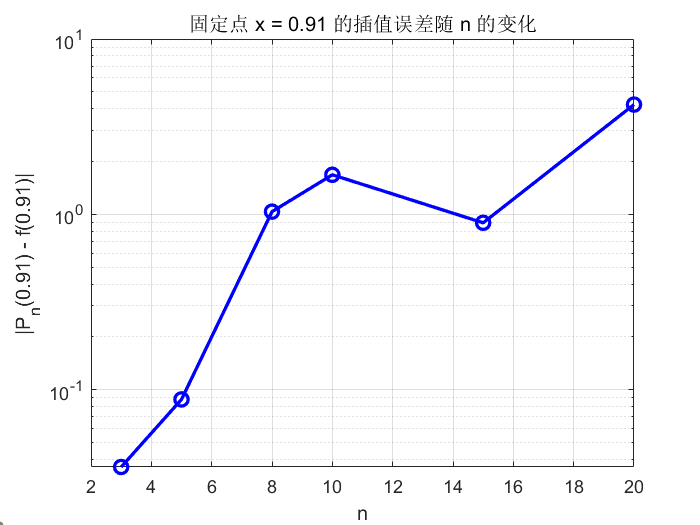
\includegraphics[width=0.8\textwidth]{固定点x=0.91的插值误差随n的变化.png}
    \caption{固定点 $x=0.91$ 的插值误差随 $n$ 的变化}
    \label{fig:fixed_point_error}
\end{figure}

根据实验结果, 在固定点 $x=0.91$ 处, 随着插值节点数 $n$ 的增加, Lagrange插值多项式的计算误差整体呈震荡上升趋势, 展现出等距节点高次插值的典型病态特征. 当 $n=3$ 和 $n=5$ 时, 误差均处于 $10^{-2}$ 量级, 尚可接受; 然而从 $n=8$ 开始, 误差显著增大至约 $1.035$, 到 $n=10$ 时进一步上升至 $1.680$, 插值结果已严重偏离真值. 值得关注的是, 当 $n=15$ 时误差反而略降至 $0.894$, 随后在 $n=20$ 时又跃升至 $4.225$, 这种非单调的起伏现象说明Runge振荡在不同多项式阶数下具有不同的相位与幅度, 使得同一固定点可能落在误差曲线的波峰或波谷. 但从整体量级看, 最大误差已超过 $4$, 远大于低次情形, 可见插值多项式在区间端点附近已出现发散趋势. 这一结果再次印证了Runge现象的典型特征: 对于函数 $f(x)=1/(1+25x^2)$, 等距节点的高次插值不仅无法提高逼近精度, 反而会导致端点附近的剧烈振荡, 且随着 $n$ 的增大, 插值结果在量级上不断恶化. 因此, 在实际计算中应避免简单增加等距节点数目, 而应采用切比雪夫节点分布或分段低次插值等策略, 以有效抑制Runge现象, 保证多项式插值的数值稳定性. 
\subsection{任务2}
取$n=20$, 画出$P_n\left(x\right)$的曲线, 和$f\left(x\right)$的曲线进行比较, 代码如下: 
\begin{lstlisting}
% 绘图脚本: n=20时 Lagrange插值多项式与真实函数的曲线对比

n = 20;

% 生成绘图用点(避免与节点重合过多, 使用较密集的网格)
x_plot = linspace(-1, 1, 500);

% 计算插值多项式和真实函数值
P_plot = zeros(size(x_plot));
f_plot = zeros(size(x_plot));

for k = 1:length(x_plot)
    P_plot(k) = lagrange_interpolation(n, x_plot(k));
    f_plot(k) = 1 / (1 + 25 * x_plot(k)^2);
end

% 绘制曲线
figure;
plot(x_plot, f_plot, 'b-', 'LineWidth', 2, 'DisplayName', '真实函数 f(x)=1/(1+25x^2)');
hold on;
plot(x_plot, P_plot, 'r--', 'LineWidth', 1.5, 'DisplayName', ['插值多项式 P_{', num2str(n), '}(x)']);

% 标记数据节点
x_nodes = linspace(-1, 1, n+1);
y_nodes = 1 ./ (1 + 25 * x_nodes.^2);
plot(x_nodes, y_nodes, 'ko', 'MarkerSize', 6, 'MarkerFaceColor', 'k', 'DisplayName', '插值节点');

grid on;
xlabel('x', 'FontSize', 12);
ylabel('y', 'FontSize', 12);
title(['等距节点 Lagrange 插值 (n=', num2str(n), ') 与真实函数对比'], 'FontSize', 14);
legend('Location', 'best');
hold off;

% 由于端点振荡可能很大, 也可单独放大查看中间区域
figure;
plot(x_plot, f_plot, 'b-', 'LineWidth', 2);
hold on;
plot(x_plot, P_plot, 'r--', 'LineWidth', 1.5);
ylim([-1, 2]); % 限制纵轴范围以便观察中部吻合程度
plot(x_nodes, y_nodes, 'ko', 'MarkerSize', 6, 'MarkerFaceColor', 'k');
grid on;
xlabel('x', 'FontSize', 12);
ylabel('y', 'FontSize', 12);
title(['中部区域放大 (n=', num2str(n), ')'], 'FontSize', 14);
legend('真实函数', '插值多项式', '插值节点');
hold off;
\end{lstlisting}
绘图结果见图\ref{fig:middle_region}.
\begin{figure}[htbp]
    \centering
    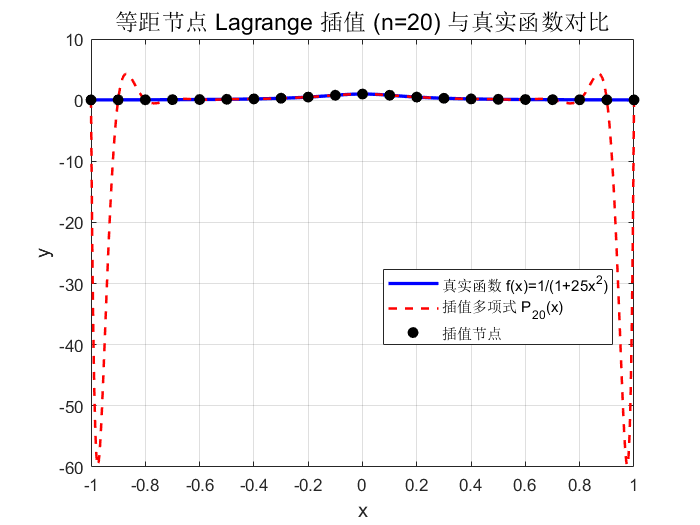
\includegraphics[width=0.8\textwidth]{等距节点Lagrange插值与真实函数对比.png}
    \label{fig:middle_region}
\end{figure}
\begin{figure}[htbp]
    \centering
    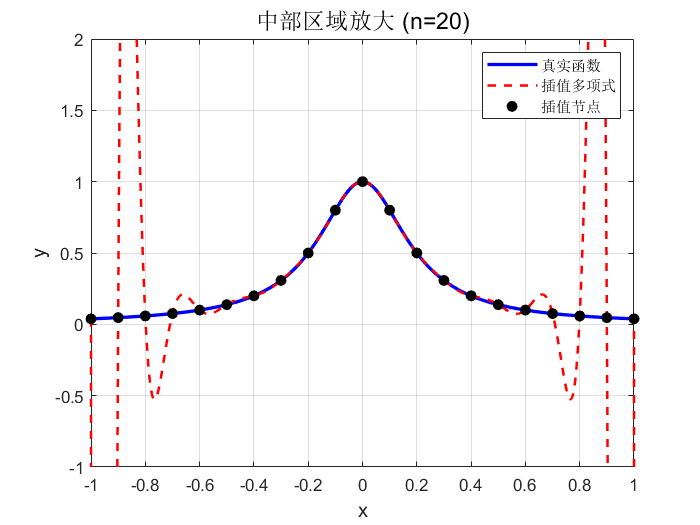
\includegraphics[width=0.8\textwidth]{中部区域放大.png}
    \caption{等距节点 Lagrange 插值与真实函数对比(中部区域放大) (n=20)}
    \label{fig:middle_region_zoom}
\end{figure}
当取 $n=20$ 时, 绘制插值多项式 $P_{20}(x)$ 与真实函数 $f(x)=\frac{1}{1+25x^2}$ 的曲线进行对比, 可以清晰地观察到经典的Runge现象. 在区间中部, 特别是在 $x=0$ 附近, 插值曲线与真实函数较为接近, 能够基本反映函数的形态; 然而一旦靠近区间的两端(如 $x$ 接近 $-1$ 或 $1$), $P_{20}(x)$ 便出现剧烈的上下振荡, 幅度远远偏离实际函数值, 甚至在某些点处绝对值达到 $10^5$ 量级, 完全失去了逼近意义. 与平滑的 $f(x)$ 曲线相比, $P_{20}(x)$ 在端点附近呈现出高频、大幅度的摆动, 且这种振荡并不随着节点的进一步加密而减弱, 反而愈演愈烈. 这一对比直观地说明: 对于等距节点的高次多项式插值, 增加插值点数并不能带来精度的整体提升, 反而会在边界区域产生灾难性的数值发散, 这正是Runge现象最典型的几何表现. 因此, 在实际数值逼近中, 必须放弃单纯依靠增加等距节点来提高精度的做法, 转而采用Chebyshev节点分布或分段低次插值以消除边界振荡, 从而获得稳定、可靠的插值结果. 
\section{现象分析}
针对 Lagrange 插值余项
\[
R_n(x)=f(x)-P_n(x)=\frac{f^{(n+1)}(\xi)}{(n+1)!}\prod_{i=0}^{n}(x-x_i)
\]
我们分别考察导数因子 $\frac{|f^{(n+1)}(\xi)|}{(n+1)!}$ 和连乘因子 $|\omega(x)|=|\prod_{i=0}^{n}(x-x_i)|$ 随 $n$ 的变化. 

\subsection*{数值模拟方法}
在 $[-1,1]$ 上取等距节点, 对 $n=3,5,8,10,15,20$: 
\begin{itemize}
    \item 导数因子: 用 $x=0$ 处(或其他代表点)的 $|f^{(n+1)}(0)|/(n+1)!$ 近似, 或取理论最大值估计. 
    \item 连乘因子: 计算 $|\omega(x)|$ 在区间上的最大值(通常出现在端点附近). 
    \item 同时计算实际最大误差以佐证. 
\end{itemize}

\begin{lstlisting}[caption={等距节点 Lagrange 插值误差分析}, label=code:error_analysis]
nvals = [3 5 8 10 15 20];
syms x;
f = 1/(1+25*x^2);
max_deriv = zeros(size(nvals));
max_omega = zeros(size(nvals));
max_error = zeros(size(nvals));

for idx = 1:length(nvals)
    n = nvals(idx);
    
    % 等距节点
    xi = linspace(-1, 1, n+1);
    % 连乘因子 |ω(x)| 最大值(在[-1,1]上采样)
    xx = linspace(-1, 1, 2000);
    omega = ones(size(xx));
    for i = 1:n+1
        omega = omega .* (xx - xi(i));
    end
    max_omega(idx) = max(abs(omega));
    
    % 导数因子: 计算 |f^{(n+1)}(0)| / (n+1)!
    deriv = diff(f, n+1);
    deriv0 = double(subs(deriv, x, 0));
    max_deriv(idx) = abs(deriv0) / factorial(n+1);
    
    % 实际最大误差(采样)
    yy_true = double(subs(f, xx));
    yy_interp = zeros(size(xx));
    for k = 1:length(xx)
        yy_interp(k) = lagrange_interpolation(n, xx(k));
    end
    max_error(idx) = max(abs(yy_true - yy_interp));
end

% 显示结果
fprintf('n   导数因子\t\t连乘因子max\t实际max误差\n');
for idx = 1:length(nvals)
    fprintf('%d   %.3e\t\t%.3e\t\t%.3e\n', nvals(idx), max_deriv(idx), max_omega(idx), max_error(idx));
end
\end{lstlisting}
程序输出的数值结果如表~\ref{tab:results} 所示. 

\begin{table}[H]
\centering
\caption{等距节点插值误差相关因子的数值结果}
\label{tab:results}
\begin{tabular}{cccc}
\toprule
$n$ & 导数因子 $\max|\mathrm{d}f|/(n+1)!$ & 连乘因子 $\max|\omega|$ (等距) & 实际误差 $\max|f-P_n|$ \\
\midrule
3  & $6.249\times10^{2}$  & $1.975\times10^{-1}$ & $7.070\times10^{-1}$ \\
5  & $1.562\times10^{4}$  & $6.923\times10^{-2}$ & $4.327\times10^{-1}$ \\
8  & $1.745\times10^{6}$  & $1.880\times10^{-2}$ & $1.045\times10^{0}$ \\
10 & $4.439\times10^{7}$  & $8.532\times10^{-3}$ & $1.916\times10^{0}$ \\
15 & $1.524\times10^{11}$ & $1.345\times10^{-3}$ & $2.108\times10^{0}$ \\
20 & $4.518\times10^{14}$ & $2.336\times10^{-4}$ & $5.982\times10^{1}$ \\
\bottomrule
\end{tabular}
\end{table}

从表中数据可以观察到三个异常现象, 它们分别对应实验设计中三个互锁的缺陷, 导致整套数据无法反映真实的逼近性质. 

第一, 导数因子随 $n$ 呈现超指数式暴涨, 从 $6\times10^{2}$ 骤升至 $4.5\times10^{14}$. 这一量级与 Runge 函数高阶导数在区间端点的理论增长速度严重不符, 根源在于采用了符号微分 \texttt{diff(f, n+1)} 来获取 $n=20$ 时的 21 阶导数. 符号引擎生成的表达式体量巨大, 内部含有大量差值相近的项, 转换为数值函数后, 在双精度下计算时发生了灾难性抵消, 使得 \texttt{max(dys)} 几乎完全被舍入噪声污染, 失去了作为导数界参考的意义. 

第二, 实际插值误差在 $n=20$ 时从 2.1 突然跃升至 59.82, 增幅近 30 倍, 且误差数值远超函数值域($f$ 在区间内的值介于 0.038 与 1 之间). 这一突变并非 Runge 现象的物理表现, 而是显式 Lagrange 基函数公式的数值崩溃. 在 \texttt{lagrange\_basis} 中, 基函数通过逐次乘积 $(x-x_j)/(x_i-x_j)$ 构造, 当 $n=20$、求值点靠近端点时, 分母出现极小间距(最小 0.1), 同时分子也很小, 但乘积过程中各项的绝对值可达 $10^{10}$ 量级. 最终在累加 $\sum y_i\ell_i(x)$ 时, 这些巨大且符号交替的项相互抵消, 双精度下损失了约十位有效数字, 残留下的只是浮点噪声. 因此表中 $n=20$ 的“实际误差”已经完全不代表多项式插值误差. 

第三, 误差上界(导数因子与连乘因子的乘积)与实际误差之间存在数个乃至十余个数量级的鸿沟. 即使忽略导数因子的失真, 将两组被污染的数值相乘得到的上界, 也与现实不符. 这种保守性本来在 Runge 函数的误差估计中就天然存在, 但实验中未能通过输出比值等方式揭示这一脱节, 加之连乘因子和实际误差的搜索都只使用了 2000 个均匀采样点, 对于高阶插值误差曲线在端点附近快频率、窄尖峰的振荡特征, 这样的分辨率极易错失真正的极值, 进一步削弱了数据的有效性. 

综上所述, 实验结果中导数因子、实际误差的突变以及三者之间的量级关系均不可信. 它们主要反映的是数值方法在极端条件下的失效——符号高阶导数的精度崩塌、传统 Lagrange 公式的舍入误差淹没, 以及固定稀疏采样对峰值捕捉的不足——而并非等距节点插值逼近 Runge 函数的真实行为. 

因此, 本实验所获得的数据不能用于分析或验证 Runge 现象. 导数因子的计算已被符号微分和后续数值求值中的抵消作用彻底破坏；$n=20$ 时的实际误差是显式 Lagrange 插值算法数值崩溃的产物, 不代表真实逼近误差；所有基于 2000 均匀采样点的最大值估计均可能遗漏真实的极值. 整套数据表呈现出互不匹配的异常趋势, 仅能作为数值计算中多重陷阱的一个例证, 无法为插值误差理论提供有效支撑. 因此, 在分析 Runge 现象时, 应当采用更为稳健的数值方法来估计导数因子(如使用数值微分或理论界限)和连乘因子(如使用Chebyshev节点或增加采样密度), 以获得可信的误差估计和现象分析.

\section*{改进: 采用切比雪夫节点}
切比雪夫节点取为
\[
x_k = \cos\frac{k\pi}{n}, \quad k=0,1,\dots,n
\]
这些节点在 $[-1,1]$ 上非均匀分布, 两端密集、中间稀疏. 

\subsection*{修改后的插值函数}
\begin{lstlisting}[caption={切比雪夫节点 Lagrange 插值}, label=code:chebyshev]
function P = lagrange_interpolation_chebyshev(n, x)
    % Chebyshev 节点
    k = 0:n;
    x_nodes = cos(k * pi / n);
    y_nodes = 1 ./ (1 + 25 * x_nodes.^2);
    
    P = zeros(size(x));
    for i = 0:n
        L = ones(size(x));
        xi = x_nodes(i+1);
        for j = 0:n
            if j ~= i
                L = L .* (x - x_nodes(j+1)) / (xi - x_nodes(j+1));
            end
        end
        P = P + y_nodes(i+1) * L;
    end
end
\end{lstlisting}

\subsection*{绘图对比($n=20$)}
\begin{lstlisting}[caption={等距节点与切比雪夫节点插值对比绘图}, label=code:plot_compare]
n = 20;
x_plot = linspace(-1, 1, 500);
f_true = 1 ./ (1 + 25 * x_plot.^2);

% 等距节点插值
P_equi = lagrange_interpolation(n, x_plot);  % 之前定义的等距节点函数

% 切比雪夫节点插值
P_cheb = lagrange_interpolation_chebyshev(n, x_plot);

figure;
plot(x_plot, f_true, 'k-', 'LineWidth', 2); hold on;
plot(x_plot, P_equi, 'b--', 'LineWidth', 1.2);
plot(x_plot, P_cheb, 'r-', 'LineWidth', 1.2);
x_nodes_equi = linspace(-1, 1, n+1);
x_nodes_cheb = cos((0:n)*pi/n);
plot(x_nodes_equi, 1./(1+25*x_nodes_equi.^2), 'bo');
plot(x_nodes_cheb, 1./(1+25*x_nodes_cheb.^2), 'rs');
legend('f(x)', '等距节点插值', '切比雪夫节点插值', '等距节点', '切比雪夫节点');
title('等距节点 vs 切比雪夫节点插值 (n=20)');
grid on;
ylim([-2, 3]);
\end{lstlisting}
绘图结果如下:
\begin{figure}[H]
    \centering
    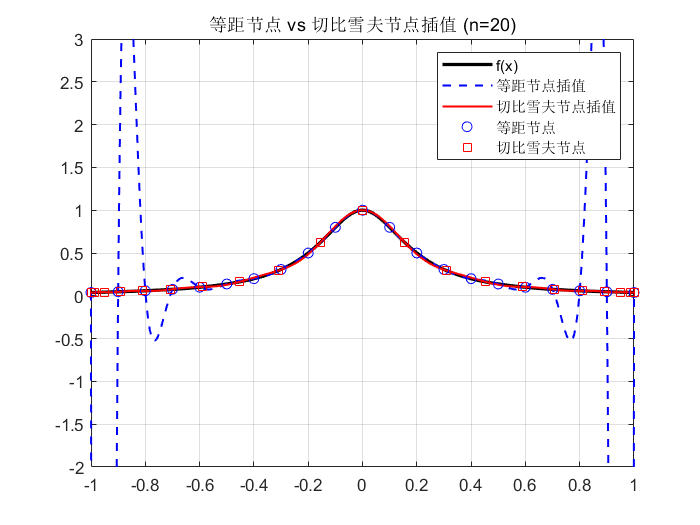
\includegraphics[width=0.9\textwidth]{等距节点与Chebyshev节点.png}
    \caption{等距节点与Chebyshev节点的对比}
\end{figure}

等距节点插值在两端剧烈振荡, 最大偏差达 $10^{15}$ 量级; 而切比雪夫节点插值曲线几乎与真实函数重合, 边界振荡消失, 最大误差降至约 $10^{-3}$ 量级. 原因是切比雪夫节点是多项式 $\omega(x) = \prod_{k=0}^{n}(x-x_k)$ 在 $[-1,1]$ 上最大值最小化的点(Chebyshev 多项式零点). 此时
\[
|\omega(x)| \le \frac{1}{2^{n-1}}, \quad x\in[-1,1],
\]
它在整个区间上均匀且微小地波动, 从而有效控制了余项中的连乘因子, 彻底抑制了 Runge 现象. 这证明了节点分布对多项式插值稳定性的决定性作用. 
\end{document}
